\documentclass[a4paper]{article} 
\usepackage{graphicx}
\graphicspath{ {./images/} }

\input{head}
\begin{document}
	
	%-------------------------------
	%	TITLE SECTION
	%-------------------------------
	
	\fancyhead[C]{}
	\hrule \medskip % Upper rule
	\begin{minipage}{0.295\textwidth} 
		\raggedright
		\footnotesize
		  Sharif University of Technology \hfill\\   
		Computer Engineering Department\hfill\\
		Ali Sharifi-Zarchi
            %\begin{figure}
    	%	\includegraphics{SharifEngLogo.png}
    	% \end{figure}
	\end{minipage}
	\begin{minipage}{0.4\textwidth} 
		\centering 
		\large 
		Homework Assignment 1\\ 
		\normalsize 
		Machine Learning for Bioinformatics, Spring 2023\\ 
	\end{minipage}
	\begin{minipage}{0.295\textwidth} 
		\raggedleft
		\small
            1401-12-11
            \hfill\\
	\end{minipage}
	\medskip\hrule 
	\bigskip
	
	%-------------------------------
	%	CONTENTS
	%-------------------------------

        %----------------------Name of the authors---------------
        \begin{center}
         Ali Shafiei, Fakhredin Abdi
        \end{center}
         %-----------------------Part 1-------------------------

        \section{Linear Regression}
        Given n training data with m features, let the target value vector be $y = [y^{(0)},...,y^{(n)}] \in \mathbb{R}^n$
        and data samples be $X = [x^{(0)};...;x^{(n)}] \in \mathbb{R}^{n\times m}$. In this context, $x_j$ denotes the jth column of this matrix.
        
        \subsection{}
        Show that if we train the regressor on just one of the features (from m features), we then have: $$w_j=\frac{x_j^Ty}{x_j^Tx_j}$$
        
        \subsection{}
        Suppose that the columns of matrix X are orthogonal. Prove that the optimal parameters from training the regressor on all features are the same as the optimal parameters resulting from training on each feature independently.
        
        \section{PCA}
        Suppose we do PCA, projecting each
        $x_i$ into $z_i$ = $V_{1:k}^Tx_i$ where 
        $V_{1:k}=[v_1,...,v_k]$, i.e., the first k principal components. We can reconstruct $x_i$ from $z_i$ as $\hat{x_i} = V_{1:k}z_i$.
        \subsection{}
        Show that $\lVert \hat{x_i}- \hat{x_j} \rVert= \lVert z_i- z_j \rVert$ .
        \subsection{}
        Show that the error in the reconstruction equals:
        \begin{align*}
\Sigma_{i=1}^n \lVert {x_i}- \hat{x_i} \rVert_2^2=(n-1)\Sigma_{j=k+1}^p \lambda_j
        \end{align*}
        where $\lambda_{k+1},...,\lambda_p$ are the p-k smallest eigenvalues. Thus, the more principal components we use for the reconstruction, the more accurate it is. Further, using the top k principal components is optimal in the sense of the least reconstruction error.

       \section{K-means}
        Perform K-means on the dataset given below. Circles are data points and there are two initial cluster centers, at data points shown with squares.
        
        \subsection{}
        Draw the cluster centers (as squares) and the decision
        boundaries that define each cluster. Use as many of the pictures as you need for convergence.      
        \newline
        \begin{center}
         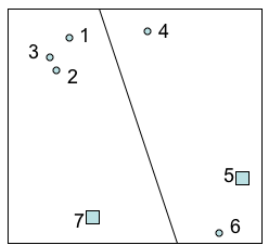
\includegraphics[scale=1]{images/question3.png}
        \end{center}
        \subsection{}
        What is the advantage of hierarchical clustering and K-means over each other (one item for each)?

        \section{Gaussian Mixture Model (GMM)}
        Suppose that our GMM is a mixture of two Gaussians: 
        $$p(x) = \pi_0N(\mu_0, \sigma_0I)+(1-\pi_0)N(\mu_1, \sigma_1I)$$
        
        \subsection{}
        Consider the set of training data below, and two clustering algorithms: K-Means, and GMM using EM (Expectation Maximization). Will these algorithms produce the same cluster centers?
        \newline
        \begin{center}
         
\includegraphics[scale=1]{images/question4.png}
        \end{center}

        \subsection{}
         Consider applying EM to train a Gaussian Mixture Model (GMM) to cluster the data
        below into two clusters. The ’+’ points indicate the current means $\mu_0$ and $\mu_1$ of the
        two Gaussian mixture components after the k-th iteration of EM.
        \newline
        \begin{center}
         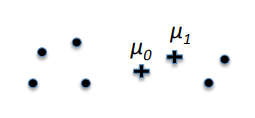
\includegraphics[scale=1]{images/question4_2.png}
        \end{center}
        
        \subsubsection{}
        In which direction $\mu_0$ and $\mu_1$ will move during the next M-step?
        \subsubsection{}
        Will the marginal likelihood of data, increase or decrease on the next EM iteration?
        
        
\end{document}
